\documentclass[pdflatex,compress]{beamer}

%\usetheme[dark,framenumber,totalframenumber]{ElektroITK}
\usetheme[darktitle,framenumber,totalframenumber]{ElektroITK}

\usepackage{graphicx}

\title{PEMODELAN JARINGAN KOMUNIKASI}
\subtitle{OSI Layer 3 - The Network Layer}

\author{Mifta Nur Farid, S.T., M.T.}

\begin{document}

\maketitle

\section{The IP Header}

\begin{frame}
	\frametitle{Layer 3 – The Network Layer}
	\begin{itemize}
		\item The Network layer is responsible for routing packets to their destination and for Quality of Service.
		\item IP (Internet Protocol) is the best known Layer 3 protocol. IPv4 is the focus of this section.
		\item It is a connectionless protocol with no acknowledgements at Layer 3.
		\item Other Layer 3 protocols include ICMP (Internet Control Message Protocol) and IPSec.
	\end{itemize}
\end{frame}

\begin{frame}
	\frametitle{IP Addressing}
	\begin{itemize}
		\item IP addressing is a logical addressing scheme which is implemented at Layer 3.
		\item The network designer uses IP addressing to partition the overall network into smaller ‘subnets’.
		\item This improves performance and security and makes troubleshooting easier.
		\item Layer 2 MAC addresses use one big flat addressing scheme. There is no logical separation between networks at Layer 2, it’s done at Layer 3.
	\end{itemize}
\end{frame}

\begin{frame}
	\frametitle{OSI Reference Model - Encapsulation}
	\begin{center}
		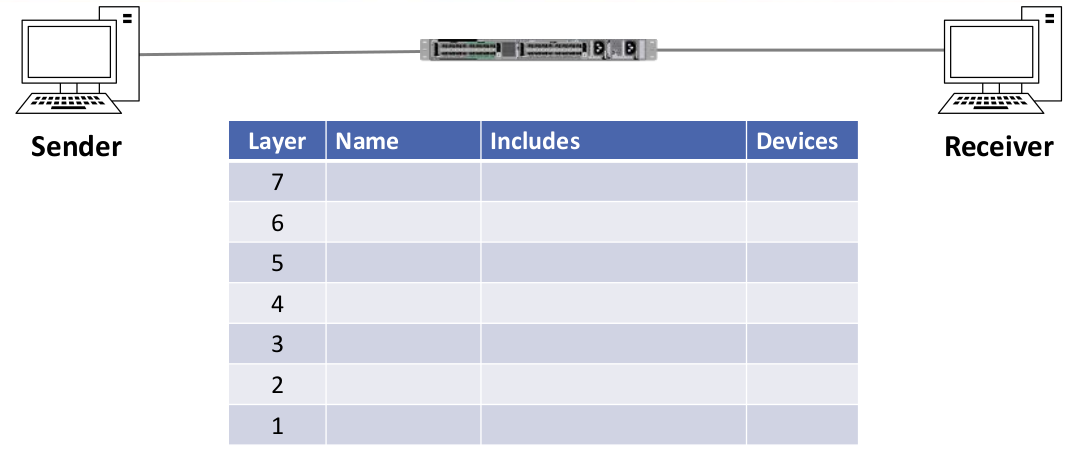
\includegraphics[width=\linewidth]{img/img01}
	\end{center}
\end{frame}

\begin{frame}
	\frametitle{OSI Reference Model - Encapsulation}
	\begin{center}
		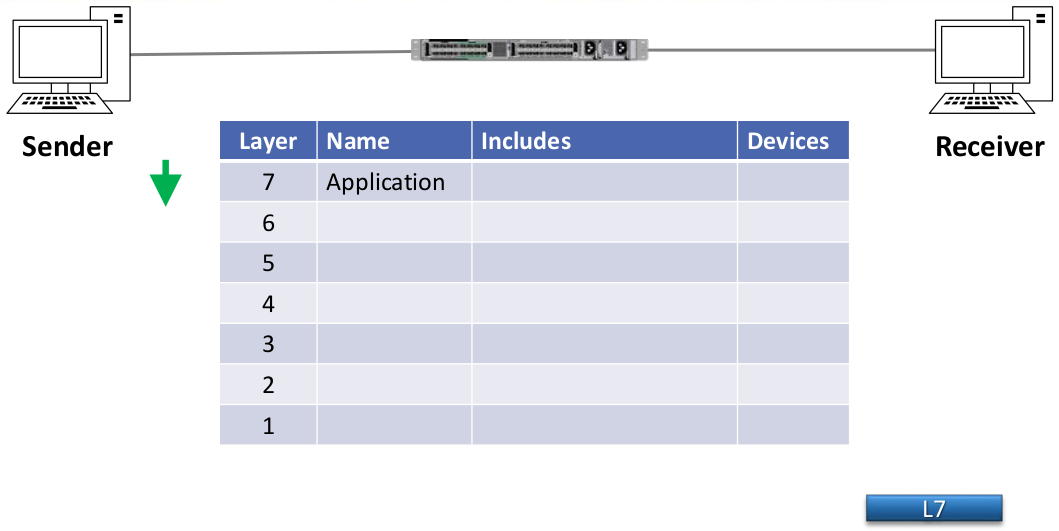
\includegraphics[width=\linewidth]{img/img02}
	\end{center}
\end{frame}

\begin{frame}
	\frametitle{OSI Reference Model - Encapsulation}
	\begin{center}
		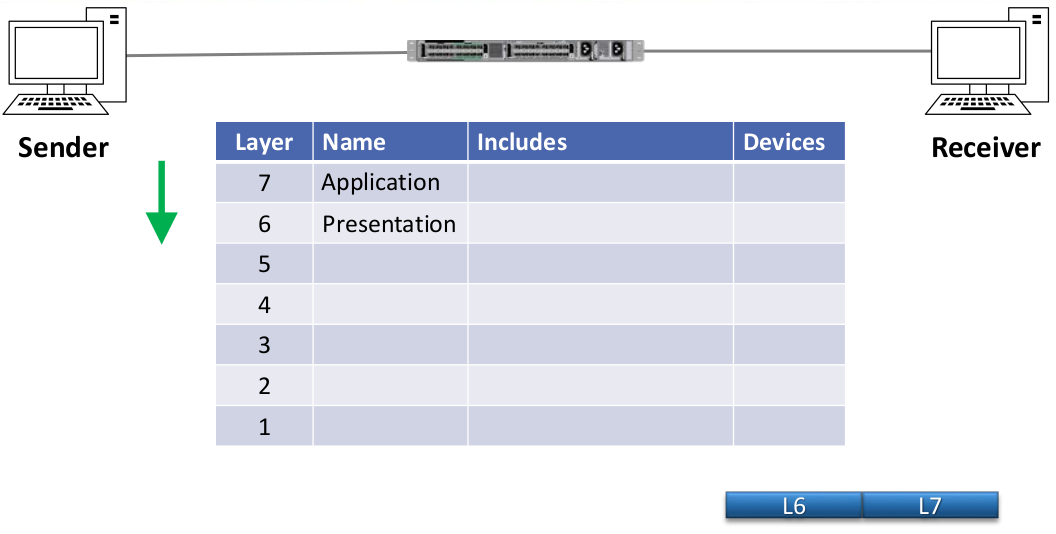
\includegraphics[width=\linewidth]{img/img03}
	\end{center}
\end{frame}

\begin{frame}
	\frametitle{OSI Reference Model - Encapsulation}
	\begin{center}
		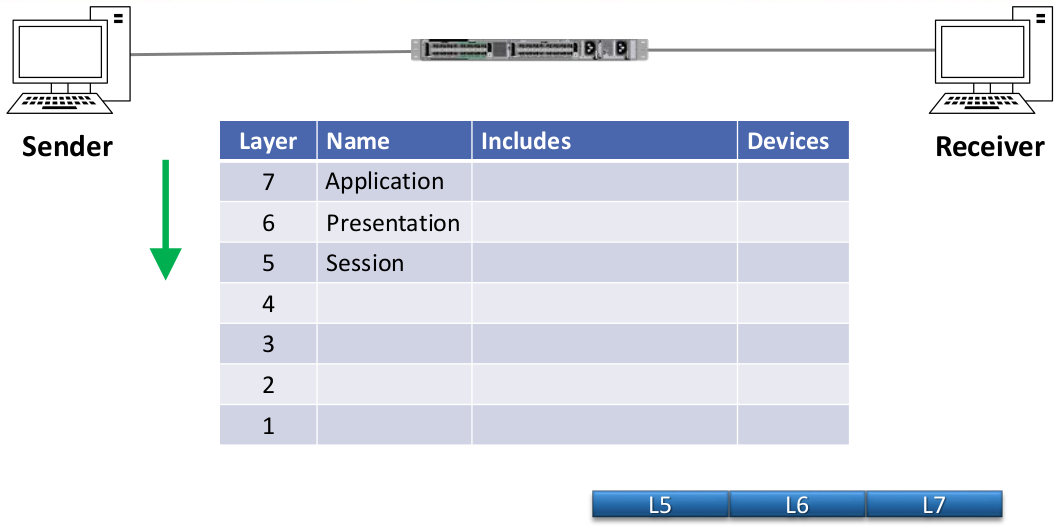
\includegraphics[width=\linewidth]{img/img04}
	\end{center}
\end{frame}

\begin{frame}
	\frametitle{OSI Reference Model - Encapsulation}
	\begin{center}
		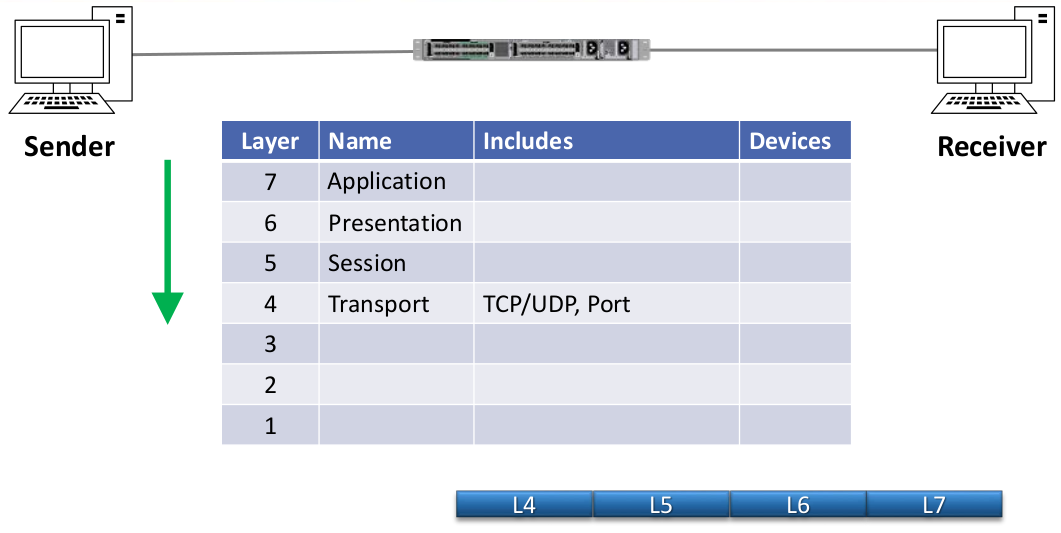
\includegraphics[width=\linewidth]{img/img05}
	\end{center}
\end{frame}

\begin{frame}
	\frametitle{OSI Reference Model - Encapsulation}
	\begin{center}
		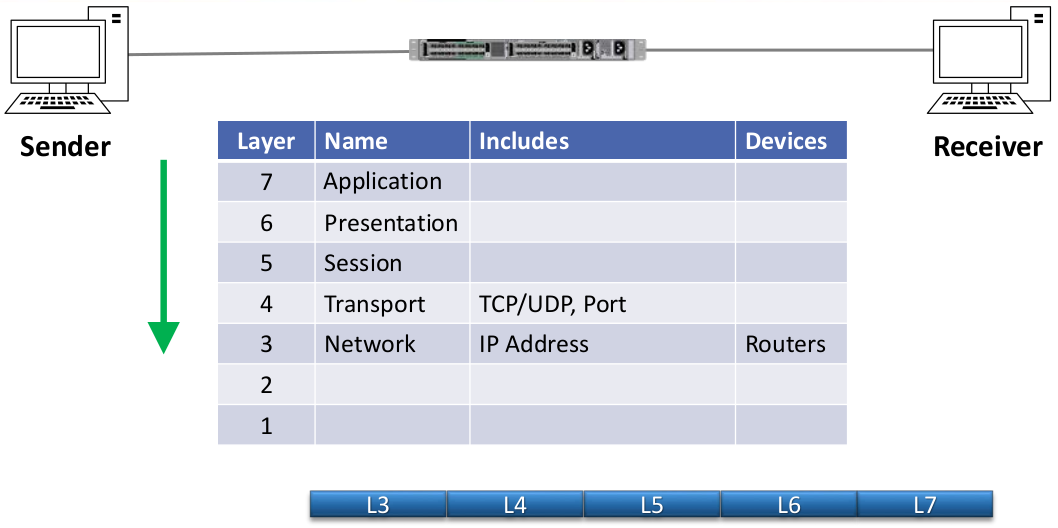
\includegraphics[width=\linewidth]{img/img06}
	\end{center}
\end{frame}

\begin{frame}
	\frametitle{OSI Reference Model - Encapsulation}
	\begin{center}
		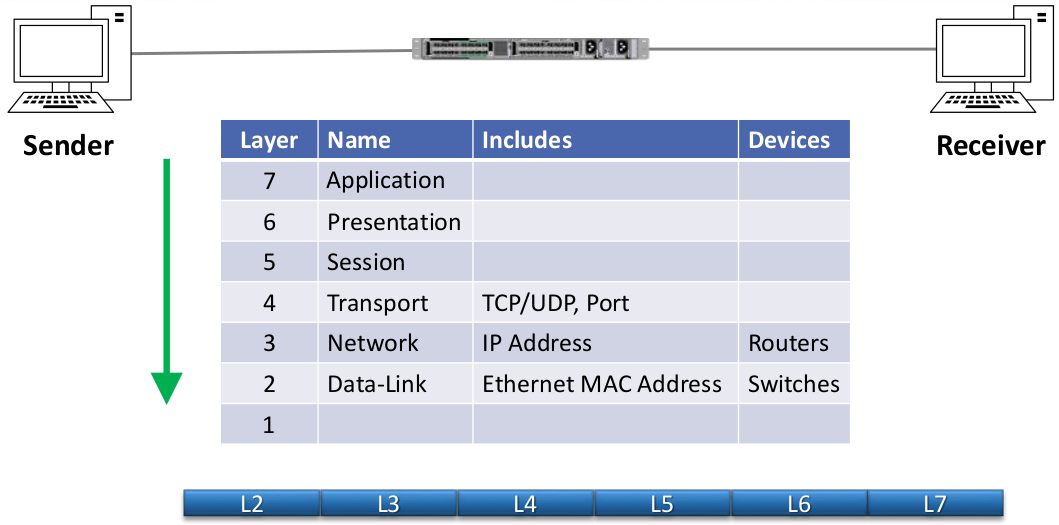
\includegraphics[width=\linewidth]{img/img07}
	\end{center}
\end{frame}

\begin{frame}
	\frametitle{OSI Reference Model - Encapsulation}
	\begin{center}
		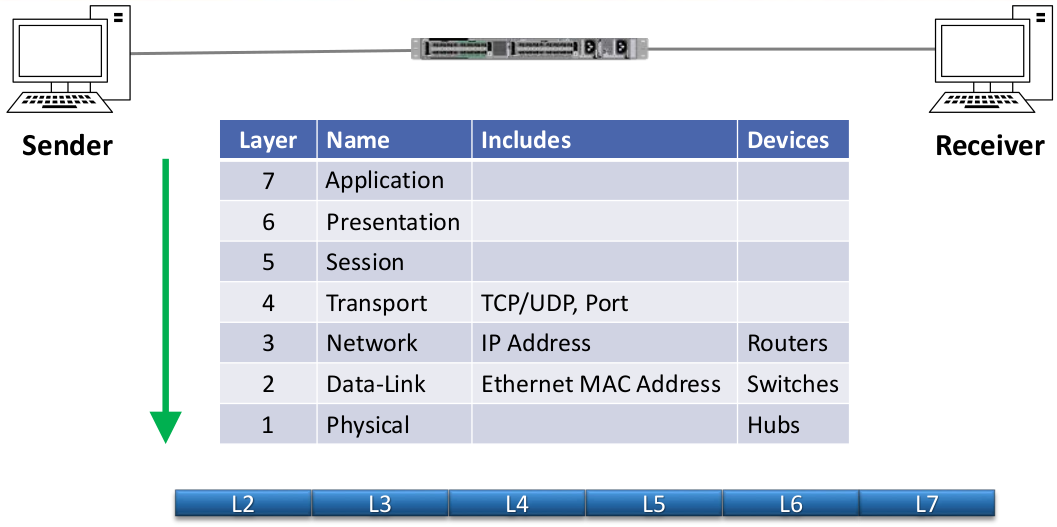
\includegraphics[width=\linewidth]{img/img08}
	\end{center}
\end{frame}

\begin{frame}
	\frametitle{The IP Header}
	\begin{center}
		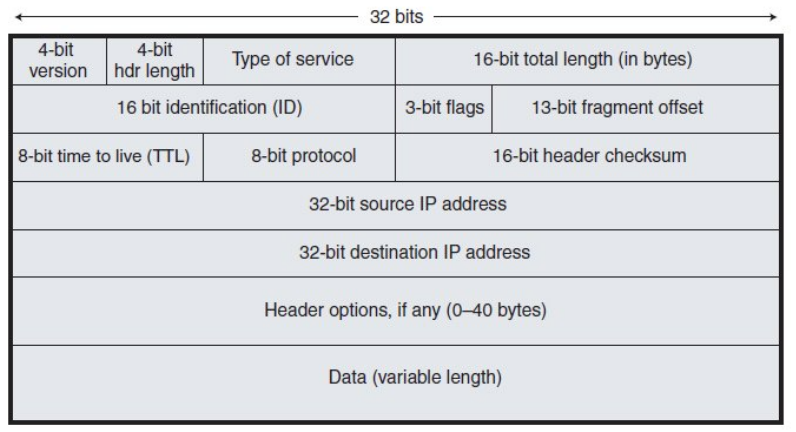
\includegraphics[width=\linewidth]{img/img09}
	\end{center}
\end{frame}

\section{Unicast, Broadcast and Multicast Traffic}

\begin{frame}
	\frametitle{Unicast, Broadcast and Multicast \\Traffic}
	\begin{itemize}
		\item There are 3 main IP traffic types: unicast, broadcast and multicast.
		\item Unicast traffic is to a single destination host.
		\item Broadcast traffic is to all hosts on the subnet.
		\item Multicast traffic is to multiple interested hosts.
	\end{itemize}
\end{frame}

\begin{frame}
	\frametitle{Unicast Traffic}
	\begin{center}
		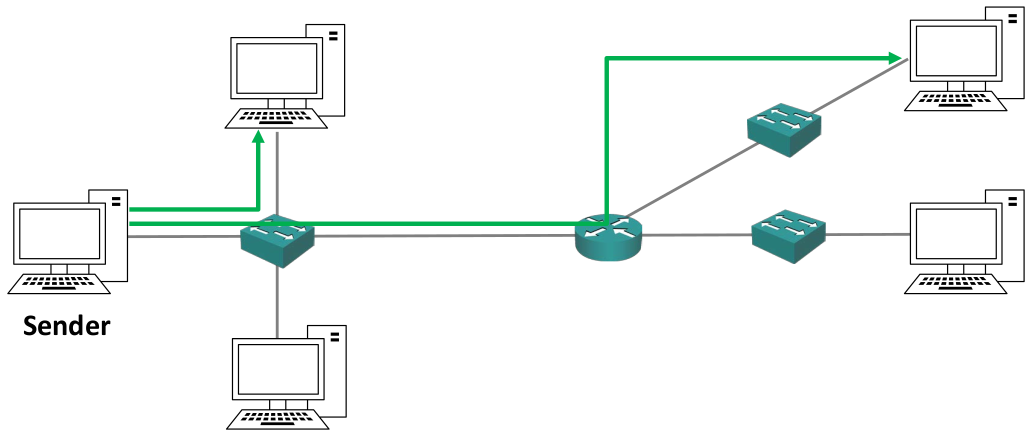
\includegraphics[width=\linewidth]{img/img10}
	\end{center}
\end{frame}

\begin{frame}
	\frametitle{Broadcast Traffic}
	\begin{center}
		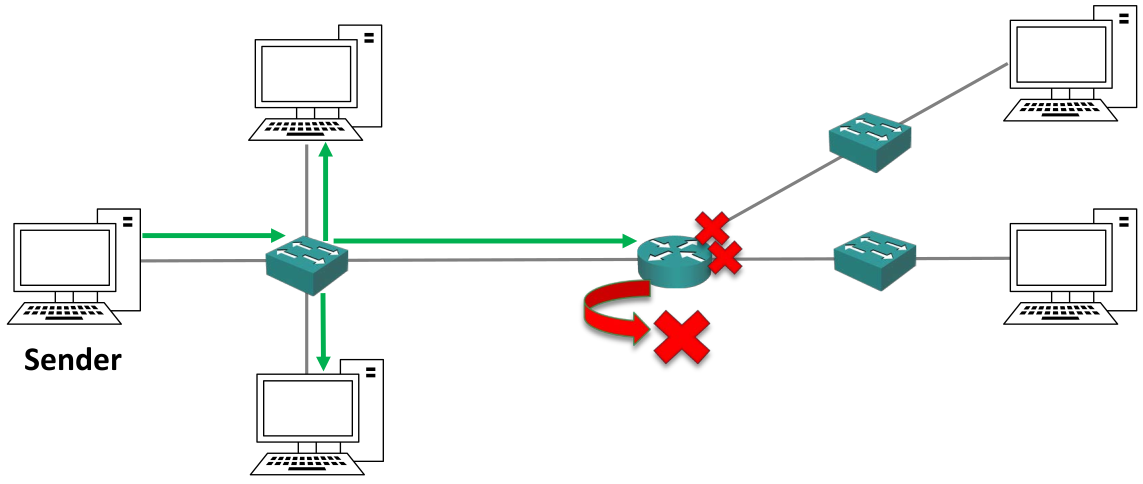
\includegraphics[width=\linewidth]{img/img11}
	\end{center}
\end{frame}

\begin{frame}
	\frametitle{Unicast Traffic to Multiple Hosts}
	\begin{center}
		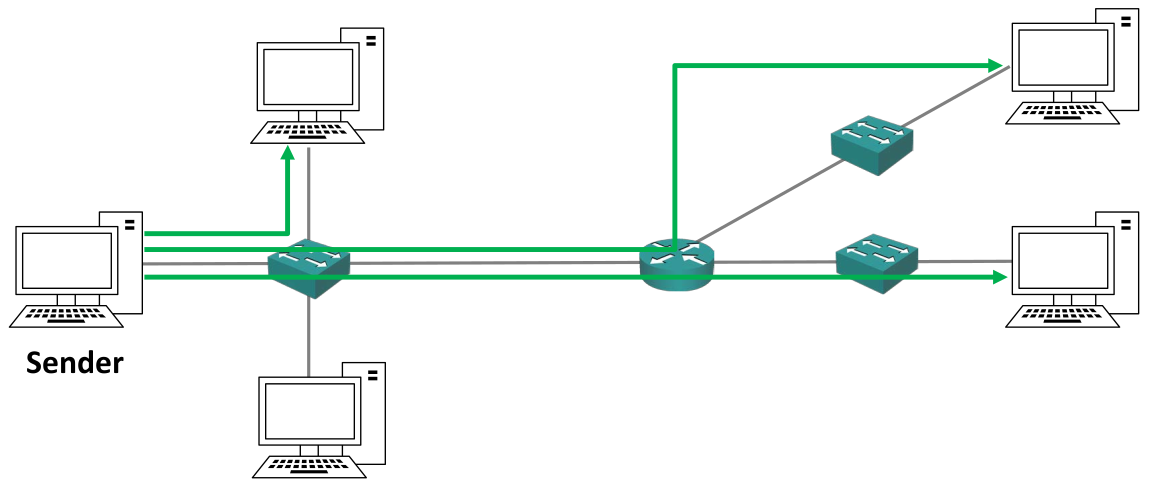
\includegraphics[width=\linewidth]{img/img12}
	\end{center}
\end{frame}

\begin{frame}
	\frametitle{Multicast Traffic}
	\begin{center}
		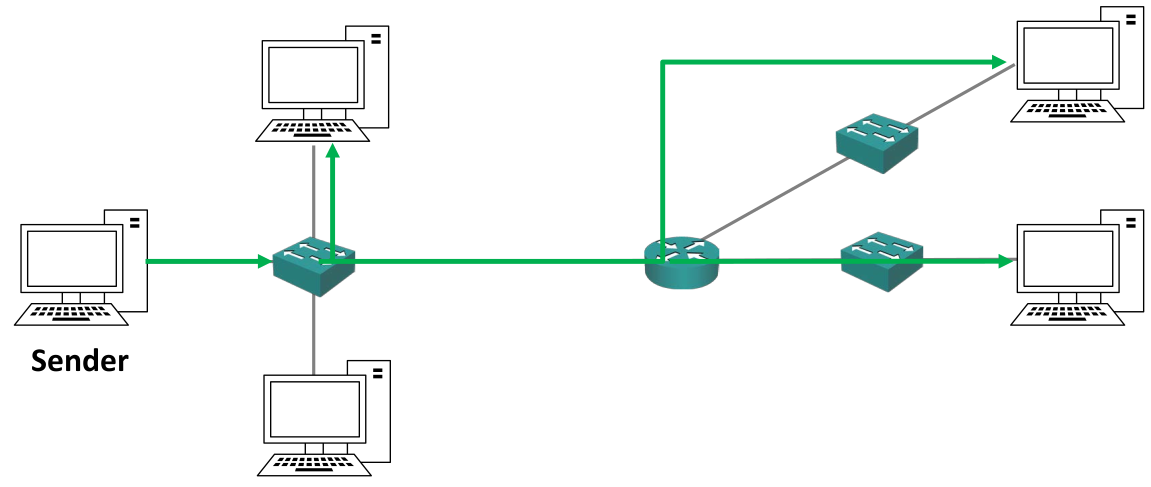
\includegraphics[width=\linewidth]{img/img13}
	\end{center}
\end{frame}

\section{Converting from Decimal to Binary}

\begin{frame}
	\frametitle{Counting in Decimal}
	\begin{itemize}
		\item Humans are conditioned to count in decimal.
		\item For each ‘column’ in a number we have 10 possible choices, from 0 to 9.
		\item Every time we add a column to the left, the value is multiplied by 10.
		\item We start with ‘1s’ as the furthest right column.
	\end{itemize}
	\begin{center}
		
\includegraphics[width=0.5\linewidth]{img/img14}
	\end{center}
\end{frame}

\begin{frame}
	\frametitle{Counting in Decimal}
	\begin{itemize}
		\item 236 is two 100’s, three 10’s, and six 1’s.
	\end{itemize}
	\begin{center}
		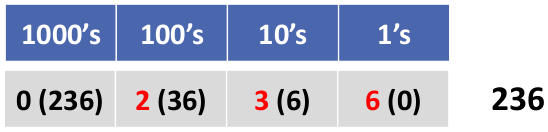
\includegraphics[width=0.6\linewidth]{img/img15}
	\end{center}
\end{frame}

\begin{frame}
	\frametitle{Counting in Binary}
	\begin{itemize}
		\item Computers work in binary.
		\item Electrical impulses are either off or on, so there’s only two choices (0 or 1), unlike 10 in decimal (0 to 9).
		\item For each ‘column’ in a number we have 2 possible choices, 0 or 1.
		\item Every time we add a column to the left, the value is multiplied by 2.
	\end{itemize}
	\begin{center}
		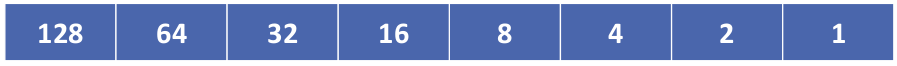
\includegraphics[width=0.8\linewidth]{img/img16}
	\end{center}
\end{frame}

\begin{frame}
	\frametitle{Counting in Binary}
	\begin{itemize}
		\item 236 in binary is 11101100
	\end{itemize}
	\begin{center}
		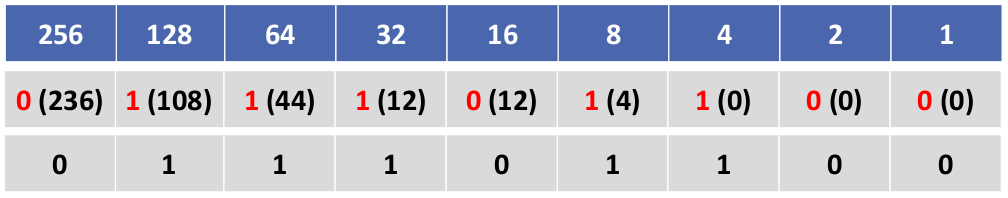
\includegraphics[width=0.9\linewidth]{img/img17}
	\end{center}
\end{frame}

\begin{frame}
	\frametitle{Counting in Binary}
	\begin{itemize}
		\item What is 179 in binary?
	\end{itemize}
	\begin{center}
		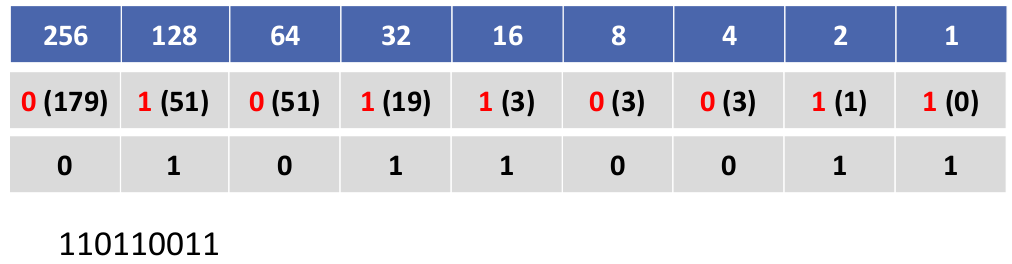
\includegraphics[width=0.9\linewidth]{img/img18}
	\end{center}
\end{frame}

\section{IPv4 Addresses}

\begin{frame}
	\frametitle{IPv4 Addresses}
	\begin{itemize}
		\item An IPv4 address is 32 bits long.
		\item It is written as 4 ‘octets’ in dotted decimal format.
		\item For example 192.168.10.15
		\item Each octet is 8 bits long $ (4 \times 8 = 32) $
	\end{itemize}	
\end{frame}

\begin{frame}
	\frametitle{Static vs Automatic Addressing}
	\begin{itemize}
		\item The IP address is usually set manually on servers, printers and network devices such as routers and switches. It is usually assigned automatically through the Dynamic Host Configuration Protocol (DHCP) on desktop computers.
		\item To understand how the logical separation between subnets works, you need to understand the IP address in binary.
	\end{itemize}	
\end{frame}

\section{Calculating an IPv4 Address in Binary}

\begin{frame}
	\frametitle{IPv4 Address Octets}
	\begin{itemize}
		\item Each octet in the IP address has a value ranging from 0 to 255
	\end{itemize}
	\begin{center}
		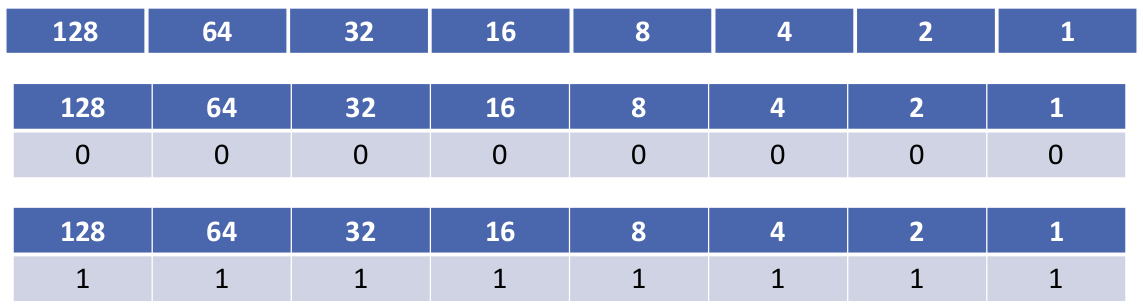
\includegraphics[width=0.9\linewidth]{img/img19}
	\end{center}
\end{frame}

\begin{frame}
	\frametitle{Converting First Octet to Binary}
	\begin{itemize}
		\item Let’s convert that 192.168.10.15 address to binary, starting with the first octet of 192.
		\item Write out the binary columns on a piece of paper to do this

		\begin{center}
			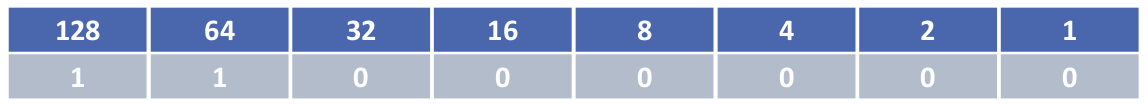
\includegraphics[width=\linewidth]{img/img20}
		\end{center}
	
		\item 192 - 128 = 64
		\item 64 - 64 = 0
		\item The first octet is 11000000 in binary
		\item 128 + 64 = 192
	\end{itemize}	
\end{frame}

\begin{frame}
	\frametitle{Converting Second Octet to Binary}
	\begin{itemize}
		\item The second octet of 192.168.10.15 is 168
		
		\begin{center}
			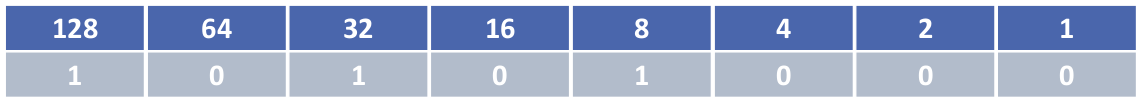
\includegraphics[width=\linewidth]{img/img21}
		\end{center}
		
		\item 168 - 128 = 40
		\item 40 - 64 doesn’t go
		\item 40 - 32 = 8
		\item 8 - 16 doesn’t go
		\item 8 - 8 = 0
		\item The second octet is 10101000 in binary
		\item 128 + 32 + 8 = 168
		\item The first half of the IP address in binary notation is 11000000.10101000
	\end{itemize}	
\end{frame}

\begin{frame}
	\frametitle{Converting Decimal to Binary}
	\begin{itemize}
		\item Go ahead and stop the video and work out the last 2 octets if you’re new to converting IP addresses to binary
		\item You should be able to show the complete IP address 192.168.10.15 in binary notation
		\item 11000000.10101000.x.x
		\item I’ll show you the answer on the next slide
	\end{itemize}	
\end{frame}

\begin{frame}
	\frametitle{Conversion Answer}
	\begin{itemize}
		\item 192.168.10.15 = 11000000.10101000.00001010.00001111
		\begin{center}
			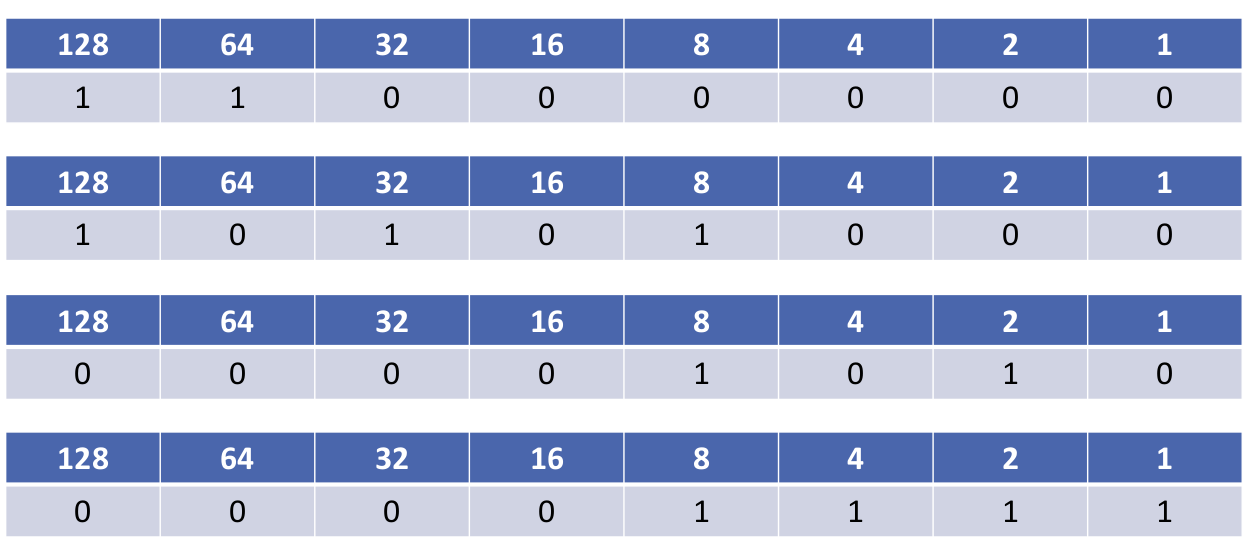
\includegraphics[width=\linewidth]{img/img22}
		\end{center}
	\end{itemize}
\end{frame}

\begin{frame}
	\frametitle{Subnet Masks}
	\begin{itemize}
		\item To set the boundary between logical networks (subnets), the IP address is combined with a subnet mask
		\item You’ll learn about the subnet mask in the next lecture
	\end{itemize}
\end{frame}

\section{The Subnet Mask}

\begin{frame}
	\frametitle{The Subnet Mask}
	\begin{itemize}
		\item A host can send traffic directly to another host on the same subnet via switches
		\item For a host to send traffic to another host in a different subnet, it must be forwarded by a router
		\item The host therefore needs to understand if the destination is on the same or a different subnet in order to know how to send it
		\item The subnet mask is used for this
		\item The subnet mask is also 32 bits long, and can be written in dotted decimal or slash notation
	\end{itemize}
\end{frame}

\begin{frame}
	\frametitle{Network and Host Portion}
	\begin{itemize}
		\item A host’s IP address is divided into a network portion and a host portion
		\item The subnet mask defines where the boundary is
		\item The easiest way to explain this is through example...
		\item Let’s say the host’s IP address is 192.168.10.15 and its subnet mask is 255.255.255.0
		\item We write the IP address out in binary notation, and then the subnet mask underneath
	\end{itemize}
\end{frame}

\begin{frame}
	\frametitle{Subnet 'Masking'}
	\begin{itemize}
		\item 192.168.10.15 / 255.255.255.0
	\end{itemize}
	\begin{center}
		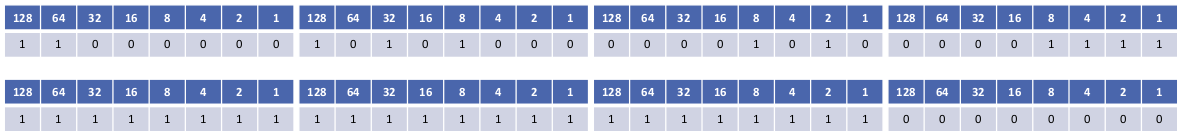
\includegraphics[width=\linewidth]{img/img23}
	\end{center}
	\begin{itemize}
		\item The IP address is compared ('masked') with the subnet mask
		\item A '1' in the subnet mask indicates that bit in the IP address is part of the network address
		\item A '0' indicates the bit is part of the host address
	\end{itemize}
\end{frame}

\begin{frame}
	\frametitle{The Network Portion}
	\begin{itemize}
		\item 192.168.10.15 / 255.255.255.0
	\end{itemize}
	\begin{center}
		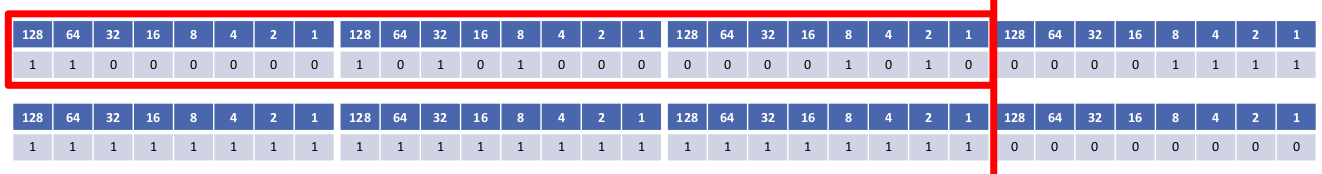
\includegraphics[width=\linewidth]{img/img24}
	\end{center}
	\begin{itemize}
		\item In our example, the network address portion is 192.168.10
		\item The host address portion is .15
	\end{itemize}
\end{frame}

\begin{frame}
	\frametitle{Local Subnet or Routed Traffic}
	\begin{itemize}
		\item 192.168.10.15 / 255.255.255.0
	\end{itemize}
	\begin{center}
		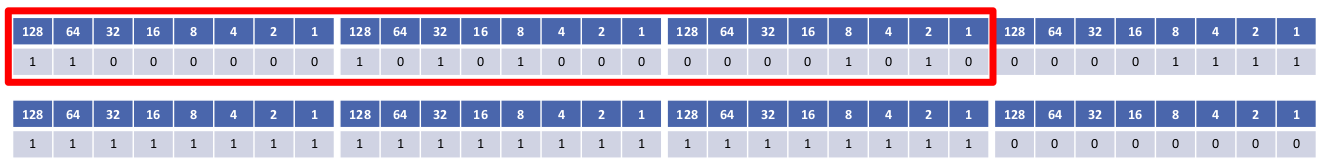
\includegraphics[width=\linewidth]{img/img25}
	\end{center}
	\begin{itemize}
		\item If the host wants to communicate with another host with an IP address which also begins with 192.168.10. (for example 192.168.10.20), it knows it’s on the
		same subnet and it can send the traffic directly
		\item If it wants to communicate with another host with any other network address (for example 192.168.11.20), it knows it has to send the traffic via a router
	\end{itemize}
\end{frame}

\begin{frame}
	\frametitle{Local Subnet or Routed Traffic}
	\begin{itemize}
		\item 192.168.10.15 / 255.255.255.0
	\end{itemize}
	\begin{center}
		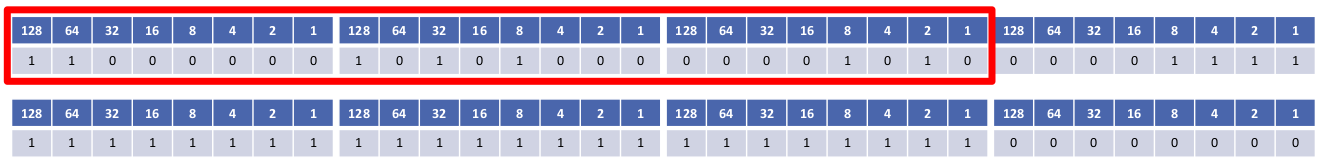
\includegraphics[width=\linewidth]{img/img26}
	\end{center}
	\begin{itemize}
		\item For a destination address to be in the same subnet, the network portion has to be \textbf{exactly} 192.168.10.
		\item Otherwise it's in a different subnet and traffic must be sent via a router
	\end{itemize}
\end{frame}

\begin{frame}
	\frametitle{Valid Subnet Masks}
	\begin{itemize}
		\item 192.168.10.15 / 255.255.255.0
	\end{itemize}
	\begin{center}
		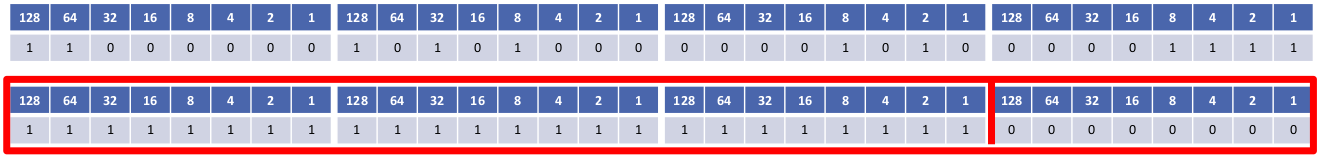
\includegraphics[width=\linewidth]{img/img27}
	\end{center}
	\begin{itemize}
		\item The subnet mask always begins with contiguous '1's
		\item For example, 11111111.11110000.00000000.00000000 is a legal subnet mask
		\item 11101101.11110000.11100000.00001111 is not
	\end{itemize}
\end{frame}

\begin{frame}
	\frametitle{The Host Portion}
	\begin{itemize}
		\item 192.168.10.15 / 255.255.255.0
	\end{itemize}
	\begin{center}
		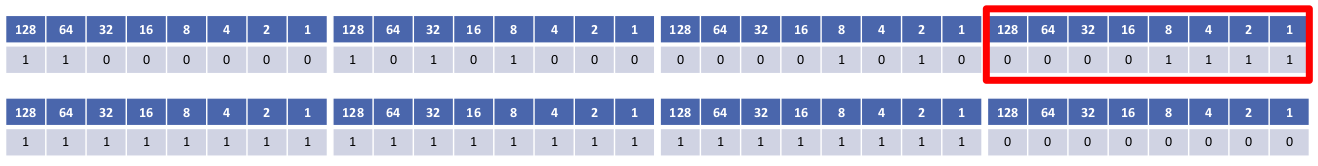
\includegraphics[width=\linewidth]{img/img28}
	\end{center}
	\begin{itemize}
		\item The host portion of the address is available to be allocated to the different hosts on the subnet (eg PCs, Servers, Printers, Router Interfaces and Switch Management Addresses)
		\item With two exceptions (coming up after the next slide)...
	\end{itemize}
\end{frame}

\begin{frame}
	\frametitle{Host Addresses}
	\begin{itemize}
		\item The host portion of the address specifies the individual host and must be unique on that subnet
		\item Hosts do not have to be numbered sequentially
		\item If the network portion of the address is 10.10.10, you can have a host with IP address 10.10.10.10 and another host with 10.10.10.20
		\item You can’t have two different hosts both with IP address 10.10.10.10. That would be a duplicate IP address. Whenever another host sent traffic to 10.10.10.10, the network wouldn’t know which one to send it to.
		\item We could have host 10.10.10.10 on one subnet and host 10.10.20.10 on another subnet
	\end{itemize}
\end{frame}

\begin{frame}
	\frametitle{The Network Address (Network ID)}
	\begin{itemize}
		\item 192.168.10.15 / 255.255.255.0
	\end{itemize}
	\begin{center}
		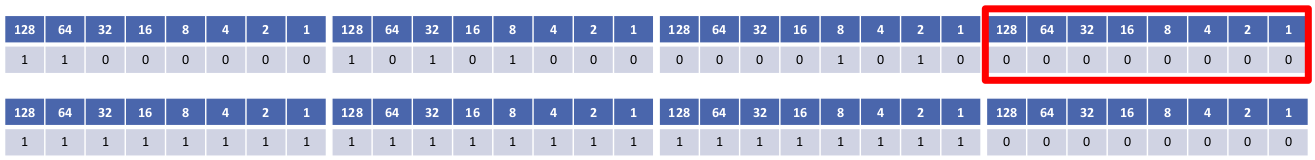
\includegraphics[width=\linewidth]{img/img29}
	\end{center}
	\begin{itemize}
		\item All 0's in the host portion designates the network address and is not allowed to be allocated to a host
		\item In our example the network address is 192.168.10.0
	\end{itemize}
	\begin{center}
		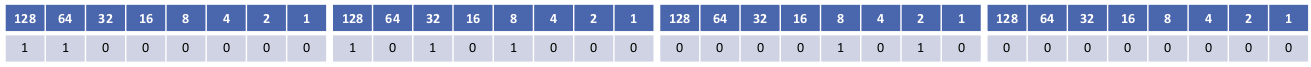
\includegraphics[width=\linewidth]{img/img30}
	\end{center}
\end{frame}

\begin{frame}
	\frametitle{The Broadcast Address}
	\begin{itemize}
		\item 192.168.10.15 / 255.255.255.0
	\end{itemize}
	\begin{center}
		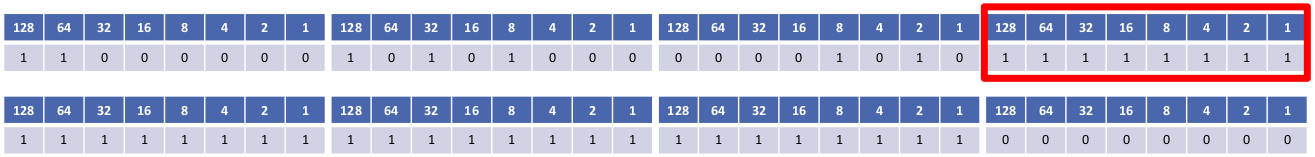
\includegraphics[width=\linewidth]{img/img31}
	\end{center}
	\begin{itemize}
		\item All 1's designates the directed broadcast address for the subnet
		\item Traffic with this destination address will be sent to all hosts in the subnet
		\item In our example the broadcast address is 192.168.10.255
	\end{itemize}
	\begin{center}
		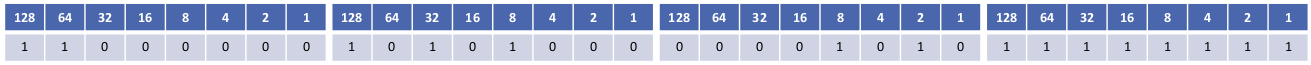
\includegraphics[width=\linewidth]{img/img32}
	\end{center}
\end{frame}

\begin{frame}
	\frametitle{Host Addresses}
	\begin{itemize}
		\item 192.168.10.15 / 255.255.255.0
	\end{itemize}
	\begin{center}
		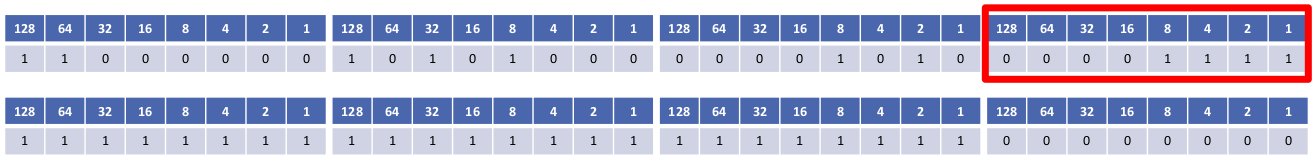
\includegraphics[width=\linewidth]{img/img33}
	\end{center}
	\begin{itemize}
		\item That leaves 192.168.10.1 to 192.168.10.254 available to be allocated to hosts
	\end{itemize}
	\begin{center}
		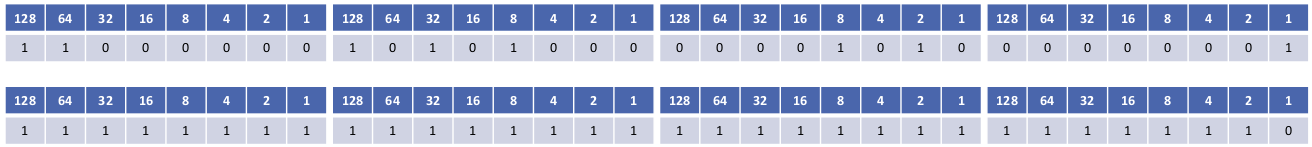
\includegraphics[width=\linewidth]{img/img34}
	\end{center}
\end{frame}

\section{Slash Notation}

\begin{frame}
	\frametitle{Subnet Mask in Slash Notation}
	\begin{itemize}
		\item 192.168.10.15 / 255.255.255.0
	\end{itemize}
	\begin{center}
		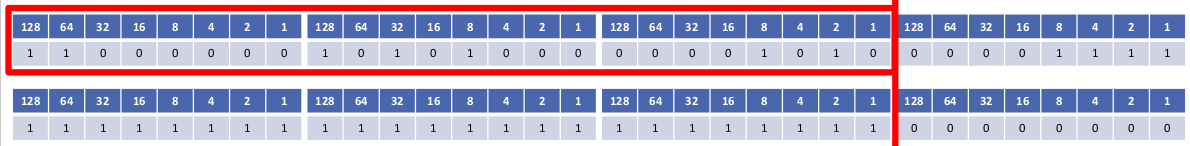
\includegraphics[width=\linewidth]{img/img35}
	\end{center}
	\begin{itemize}
		\item Because the subnet mask always begins with contiguous '1's, it will be 1 to 32 bits long counting from left to right
		\item This allows us to write the subnet mask in slash notation which is more convenient than dotted decimal for network diagrams or in conversation
	\end{itemize}
\end{frame}

\begin{frame}
	\frametitle{Subnet Mask in Slash Notation}
	\begin{itemize}
		\item 192.168.10.15 / 255.255.255.0
	\end{itemize}
	\begin{center}
		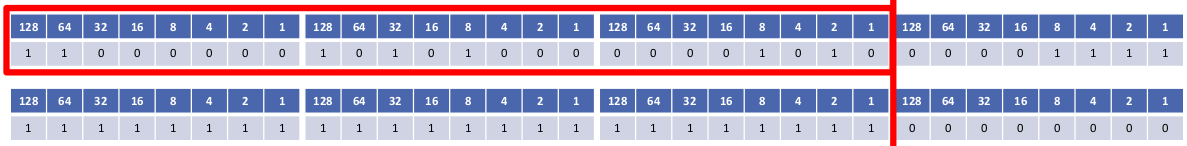
\includegraphics[width=\linewidth]{img/img36}
	\end{center}
	\begin{itemize}
		\item Our example can be written as either 192.168.10.15 255.255.255.0 or 192.168.10.15/24
		\item The network address is 192.168.10.0/24
	\end{itemize}
\end{frame}

\begin{frame}
	\frametitle{Subnet Mask in Slash Notation Example 2}
	\begin{itemize}
		\item 10.10.10.15 / 255.0.0.0
	\end{itemize}
	\begin{center}
		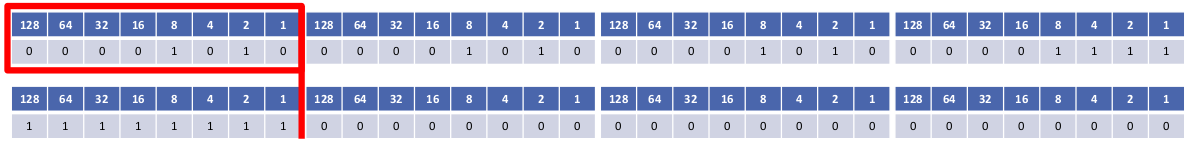
\includegraphics[width=\linewidth]{img/img37}
	\end{center}
	\begin{itemize}
		\item This example can be written as either 10.10.10.15 255.0.0.0 or 10.10.10.15/8
		\item The network address is 10.0.0.0/8
	\end{itemize}
\end{frame}

\end{document}